%%%%%%%%%%%%%%%%%%%%%%%%%%%%%%%%%%%%%%%%%
% Simple Sectioned Essay Template
% LaTeX Template
%
% This template has been downloaded from:
% http://www.latextemplates.com
%
% Note:
% The \lipsum[#] commands throughout this template generate dummy text
% to fill the template out. These commands should all be removed when 
% writing essay content.
%
%%%%%%%%%%%%%%%%%%%%%%%%%%%%%%%%%%%%%%%%%

%----------------------------------------------------------------------------------------
%	PACKAGES AND OTHER DOCUMENT CONFIGURATIONS
%----------------------------------------------------------------------------------------

\documentclass[12pt]{article} % Default font size is 12pt, it can be changed here

\usepackage{geometry} % Required to change the page size to A4
\geometry{a4paper} % Set the page size to be A4 as opposed to the default US Letter

\usepackage{graphicx} % Required for including pictures

\usepackage{float} % Allows putting an [H] in \begin{figure} to specify the exact location of the figure
\usepackage{wrapfig} % Allows in-line images such as the example fish picture

\usepackage{lipsum} % Used for inserting dummy 'Lorem ipsum' text into the template

\linespread{1.2} % Line spacing

%\setlength\parindent{0pt} % Uncomment to remove all indentation from paragraphs

\graphicspath{{Pictures/}} % Specifies the directory where pictures are stored

\begin{document}
	
	%----------------------------------------------------------------------------------------
	%	TITLE PAGE
	%----------------------------------------------------------------------------------------
	
	\begin{titlepage}
		
		\newcommand{\HRule}{\rule{\linewidth}{0.5mm}} % Defines a new command for the horizontal lines, change thickness here
		
		\center % Center everything on the page
		
		\textsc{\LARGE Wits University}\\[1.5cm] % Name of your university/college
		\textsc{\Large School of Electrical and Information Engineering}\\[0.5cm] % Major heading such as course name
		\textsc{\large ELEN7046 - Software Technologies and Techniques}\\[0.5cm] % Minor heading such as course title
		
		\HRule \\[0.4cm]
		{ \huge \bfseries Big Data Visualization using Commodity Hardware and Open Source Software}\\[0.4cm] % Title of your document
		
		Solution: Twit-Con-Pro
		
		\HRule \\[0.6cm]
		
		\begin{minipage}
			{0.4
				\textwidth} 
			\begin{flushleft}
				\large \emph{Authors:}\\
				Gareth \textsc{Stephenson} \\
				Matsobane \textsc{Khwinana} \\
				Sidwell \textsc{Mokhemisa} \\
				Dave \textsc{Cloete}\\
				Kyle \textsc{Trehaeven}
			\end{flushleft}
		\end{minipage}
		~ 
		\begin{minipage}
			{0.4
				\textwidth} 
			\begin{flushright}
				\large \emph{Student Number:} \\
				778919 \\
				779053  \\
				1229756 \\
				1573016 \\
				0602877N
				% Supervisor's Name
			\end{flushright}
		\end{minipage}
		\\[1cm]
		\
		\\
		\
		\\
		\
		
		https://github.com/garethstephenson/ELEN7046\_Group2\_2016\\
		\
		\\
		\
		\\
		\
		\\
		\
	
		{\large \today}\\[3cm] % Date, change the \today to a set date if you want to be precise
		
		%\includegraphics{Logo}\\[1cm] % Include a department/university logo - this will require the graphicx package
		
		\vfill % Fill the rest of the page with whitespace
		
	\end{titlepage}
	
		\newpage
		\begin{flushleft}\large
			\textsc{Declaration of Originality}\\
		\end{flushleft}
		
		ELEN7046 Group 2 team members hereby declare the following:
		
		\begin{itemize}
			\item We are aware that plagiarism (the use of someone else’s work without their permission and/or without acknowledging the original source) is wrong.
			\item We confirm that ALL the work submitted for assessment for the above course is our own unaided work except where we have explicitly indicated otherwise.
			\item We have followed the required conventions in referencing the thoughts and ideas of others.
			\item We understand that the University of the Witwatersrand may take disciplinary action against each one of us if there is a belief that this is not our own unaided work or that we have failed to acknowledge the source of the ideas or words in our writing.
		\end{itemize}
		
%\begin{center}
%	\begin{tabular}{ | p{3cm} | p{3cm} | p{2.5cm} | c | c |}
%				\hline
				%	\multicolumn{1}{ |l| }{Use Case ID:} & \multicolumn{3}{| l |}{UC01}\\
				%	\hline
				%	\multicolumn{1}{|l|}{Use Case Name:} & \multicolumn{3}{|p{13cm}|}{View Analytics Social Media Report overlaid on map background.}\\
				%	\hline
%				\textbf {Member Name} & \textbf {Primary Task} & \textbf {Time Spent (Hours)} & \textbf {Discretionary} & \textbf {Member Signature}  \\
%				\hline
%				Sidwell Mokhemisa & Architecture & 111 & 5 \% & \\
%				\hline
%				Kyle Trehaeven & Development - Streaming & 140 & 5 \% & \\
%				\hline
%				Matsobane Khwinana & Development - History & 118 & 5 \% & \\
%				\hline
%				Gareth Stephenson & Development - MapReduce & 205 & 5 \% & \\
%				\hline
%				Dave Cloete & Development - Visualization & 127 & 5 \% &\\
%				\hline
%			\end{tabular}
%		\end{center}
				\begin{figure}[H] % Example image
					\center{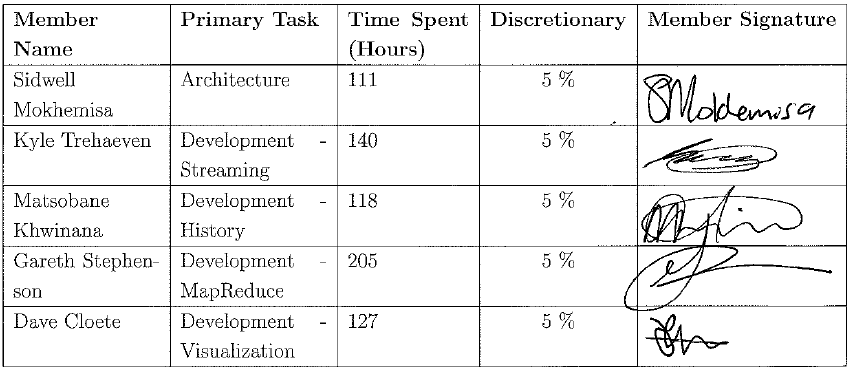
\includegraphics[width=1.15\linewidth]{Declaration}}
					%\caption{IBM Rational Unified Process (Source: RUP, Best Practices for Software Development Teams)}
					\label{fig:speciation}
				\end{figure}
		
		\pagenumbering{gobble}% Remove page numbers (and reset to 1)
		\newpage
		
		% Abstract
		\begin{flushleft}\large
			\textsc{Abstract}\\
			The project aims to provide a low cost solution to big data processing problems, enabling a commercially viable option to individuals, small businesses and academia using commodity hardware. This report explores the use of  Open Source technologies Apache Spark and Scala as well as the low cost and scalable Raspberry Pi's. After building a prototype system to source, process and visualize data from Twitter, it was concluded that  commodity hardware is a viable small-scale solution to working with Big Data.
			
		\end{flushleft}
	
		% Abstract
		
	
		\pagenumbering{gobble}% Remove page numbers (and reset to 1)
		\newpage
	
	%----------------------------------------------------------------------------------------
	%	TABLE OF CONTENTS
	%----------------------------------------------------------------------------------------
	
	\tableofcontents % Include a table of contents
	
	\newpage % Begins the essay on a new page instead of on the same page as the table of contents 
	
	\pagenumbering{arabic}% Remove page numbers (and reset to 1)

	%----------------------------------------------------------------------------------------
	%	INTRODUCTION
	%----------------------------------------------------------------------------------------
	
	\section{Introduction} % Major section
	
This report presents the work done by Group 2 in response to the project brief for ELEN7046: Software Technologies and Techniques.\\

The report will broadly focus on the following topics:

\begin{itemize}
	\item The Methodology followed to execute the project;
	\item The Architecture of the solution developed for the project; and
	\item The different technologies used to deliver the solution.
\end{itemize}

\subsection{Problem Statement}

There is an abundance of big data available to individuals and companies with very limited capacity to refine this data into meaningful information, particularly for small scale endeavours. Big Data processing is often locked behind high cost barriers to entry, and individuals, start ups and academics may find it difficult to be involved in Big Data processing.

\subsection{Solution Summary}

Commodity hardware is available to provide a means by which the barrier to entry for Big Data projects can be overcome. Simple, low cost components can be leveraged to address each of the parts of a big data processing solution, whether it be data sourcing, transormation, or visualization; and can be scaled according to needs or as required.

\subsection{Project Delivery Approach}

As the team was not co-located, challenges around communication and general collaboration was raised before the first team meeting. 
The team made use of the following, online collaboration tools to meet their needs as well as drive the project delivery:
\begin{itemize}
	\item \textbf{Trello:} To manage collaborative tasks and to provide an understanding of the scope of work.
	\item \textbf{WhatsApp:} To initiate any discussion that required an immediate response.
	\item \textbf{Slack:} For knowledge sharing and lengthy, more general discussions.
	\item \textbf{GitHub:} Source Control and Content Management.
	\item \textbf{Google Hangouts:} For collaborative, interactive knowledge sharing .
	\item \textbf{Contact Sessions:} To ensure frequent, face-to-face communication and ensuring the project moved forward, the team decided to meet every Sunday for the duration of the project. 
\end{itemize}

%\subsubsection{Methodology}
	
		%\subsection{Executive Summary} % --optional
		
		%------------------------------------------------
		
	\section{Literature Review}
	
	\subsection {Data Sourcing}
	
	This project was intended to deliver a system or solution for the visualization of Big Data. For this reason it is important that we start by defining what Big Data is.
	\\
	According to Maden[1], Big Data can be defined as "data that is too big, too fast, or too hard for existing tools to process."
	\\
	The above definition further supports our group's decision to focus on Twitter as the source of data for the project. Statistics have shown the following average figures with regards to the amount of data that one can get from Twitter[2]:
	\\
	
		\begin{itemize}
			\item 6000 per second; 
			\item 350 000 per minute;
			\item 500 million per day; and
			\item 200 billion in a year.
		\end{itemize}
	
	\subsection {Big Data Processing Algorithm}
	
	The team sought to have all the processing of the Big Data received from Twitter done on multiple nodes following the principles of MapReduce.
	\\
	\\
	Apache Spark was used for this project together with MapReduce which in the main delivers the MapReduce functionality based on the algorithm that is broken down into the Mapper class and the Reducer class[3].\\
	
	The Apache Spark cluster computing framework runs the MapReduce algorithm across all the nodes within the Raspberry Pi network, allowing for fast and efficient querying and transformation of raw data into meaningful information.
	
	\subsection{Data Visualization}
	
	Data Visualization is key to understanding large sets of data. Graphically representing  data allows the human mind to better comprehend abstracted views and makes it easier to identify trends, patterns and anomalies not easily identifiable when looking at data in more traditional forms such as spreadsheets.
		
	
		\section{Success Criteria} % Major section
		
		\begin{itemize}
			\item Build a system that uses commodity hardware to solve for big data problems;
			\item Provide a solution that covers the data sourcing, transformation and presentation of social media data from Twitter relating to the United States and South African elections. The end result must be visualization that provides insight to the sentiment of election candidates on Twitter.
		\end{itemize}
		

	
	\section{Lifecycle Methodology}
	
	%\subsection{Explanation Summary} %--optional
	
	%------------------------------------------------
	In order for the team to successfully deliver this project, a development methodology based on IBM Rational Unified Process (RUP) was followed albeit tailored to cater for the specific needs of this project.\\
	\\
	The diagram below depicts the IBM RUP model:
	
		\begin{figure}[H] % Example image
			\center{\includegraphics[width=1.15\linewidth]{ibm1}}
			\caption{IBM Rational Unified Process (Source: RUP, Best Practices for Software Development Teams)}
			\label{fig:speciation}
		\end{figure}
		
		
	
%	\subsection{info}
	
	
	%------------------------------------------------
	
%	\subsection{Observation} % Sub-section
	
	
%	\subsubsection{Value}
	
	
	%\\subsubsection{Risk}
	%--Risk categories SP03

%	\subsubsection{Cost \& Schedule}
	
\section{Key Risks}

Below is the list of the Key Risks that the project team identified at the start of the project:\\

\begin{itemize}
	\item Project Technical Risk.
	\item The Raspberry Pi Infrastructure.
	\item Team Collaboration.
\end{itemize}
	
	%\subsection{xxx}
	\section{Assumptions and Constraints}
	
\subsection{Assumptions and Acknowledgements}

\begin{itemize}
	
	
	\item It is assumed that a rudimentary algorithm for sentiment assessment is "Good Enough", forgoing complex natural language inference. 
	
	\item It is assumed that any incidental tweets sourced (such as EFF referencing the Electronic Freedom Foundation) are minimal and acceptable.
	
	\item It is assumed that Twitter is providing us with either the full extent of our search criteria, or if this is not the case, then the sample that is received is a representational slice of all data and is proportionally equivalent.
	
	\item It is assumed that information that users provide on twitter (name of their location in particular) is correct and relevant, and that those who do not are in the minority.
	
	\item Failing the above, it is assumed that of those who do provide location based information; their distribution is representative of the norm.
	
	\item It is assumed that the graphical solution provided can be rendered by any clients that access them.
	
	\item It is assumed that the datasets provided for the visualisation components will be small enough to be effectively transferred over the internet to browsers without error.
	
	\item It is acknowledged that demographics of the provided data are skewed (younger people more likely to use twitter, poorer South Africans less likely to use twitter).
	
	\item It is acknowledged that application software is not optimised extensively.
\end{itemize}

\subsection {Technical Constraints}

\begin{itemize}
	\item \textbf{Twitter API:} Twitter only provided100 tweets per request and only allowed 450 tweets within a 15 minutes window[4].
	\item \textbf{GoogleAPI:} Google has a restriction that only allows 2500 requests   per day.
	\item \textbf{Hardware:} Slow I/O processing due to cheaper storage (SD Card), limited physical space that could only accommodate just over 1,5 million tweets as well as limited RAM on the Raspberry Pi's.
\end{itemize}

	
	\section {Design Decisions}
	
	The table below details all the key design decisions made in the delivery of the solution:
	
\begin{itemize} 
	\item \textbf{History Data:} History data/ batch interface to Twitter was designed to provide past data subscribed to based on date range.
	
	\item \textbf{Streaming Data:} 
	This interface provides for all subscribed data in real-time starting from now and going into the future.
	
	One of the motivating factors for splitting the two components mentioned above was that the project followed a divide and conquer strategy to decompose
	the data collection problem into simpler sub-components. The divide and conquer strategy in software design, helps in avoiding a single point of failure, and it 
	enables parallelism [6].
	
	\item \textbf{GoogleMaps:} 
	 Where privacy settings were not enabled for current location, an interface to GoogleMaps was developed to read the location information of the person tweeting from their Twitter profile and resolve this to actual co-ordinates.
	
	\item \textbf{Security Directive(s):} 
	It was decided that where security is concerned, only the Twitter and GoogleMaps security requirements be adhered to where integration is concerned. All data acquired from Twitter is data that is already in the public domain, therefore no effort was required to secure the data while in transit, hence the use of only FTP instead of a lot more secure transport mechanism.
\end{itemize}
	
	
	
	\section{Solution Design}
		
	\subsection{High Level Design: Component Architecture}
	The high level component model below depicts the key features of the solution delivered for the project.
	\\
	\\
	This design can be categorised into the following three features from a functionality point of view:
	
		\begin{itemize}
			\item Acquiring data from Twitter based on topics subscription - Political Party sentiment in USA and RSA for 2016. This was achieved by using JEE for history and C\# for online data acquisition while persisting all data in MongoDB.
			\item Data processing was achieved using Apache Spark with MapReduce algorithms developed in Scala. Data in MongoDB was extracted and transfered via FTP to the clustered infrastructure where all the necessary transformation happened.
			\item Extracts from the transformation process were sent to the presentation tier application in JSON format where node.js was used in conjunction with D3 chartz to render the visualized big data content on a web browser.
		\end{itemize}
	
	
		\begin{figure}[H] % Example image
			\center{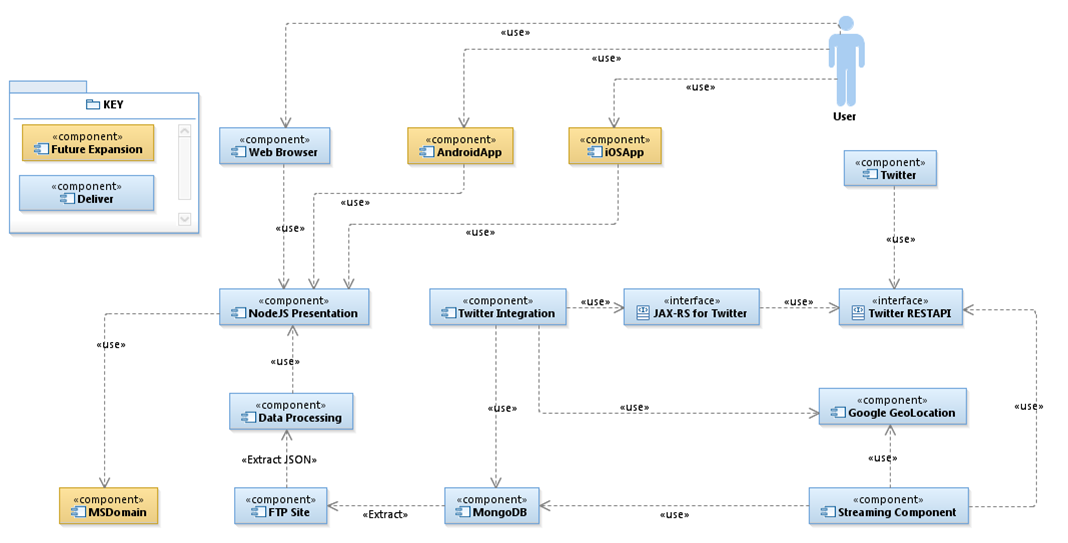
\includegraphics[width=1.15\linewidth]{HLD1}}
			\caption{High Level Component Model.}
			\label{fig:speciation}
		\end{figure}
	
	\subsection{Detailed Designs}
	
	\subsubsection{Data Acquisition (History)}
	
	The historic data collection component is made up of two major services, namely, Data Extraction Service and Data Distribution Service. These supports the two major use cases for history data collection component, i.e. data acquisition and distribution. The services were modelled using public interfaces, packaged together in the API module. The interfaces are separated from the implementations to avoid tight coupling and thereby making it easy to swap implementations without impacting the API users.
	\\
	\\
	The implementation components perform the actual extraction of the data by interacting with the Twitter REST API; in the process they perform authentication, retrieval of content, mapping the content from Twitter to the application’s Tweet entity and persisting the data in MongoDB. Similarly for the distribution of data, the underlying classes handle the retrieval of data from MongoDB and distribute the data using FTP.
	\\
	\\
	The extraction service can be triggered using both the REST interface and the Scheduler, whilst the distribution component can be triggered via the REST interface only.
	
	
		\begin{figure}[H] % Example image
			\center{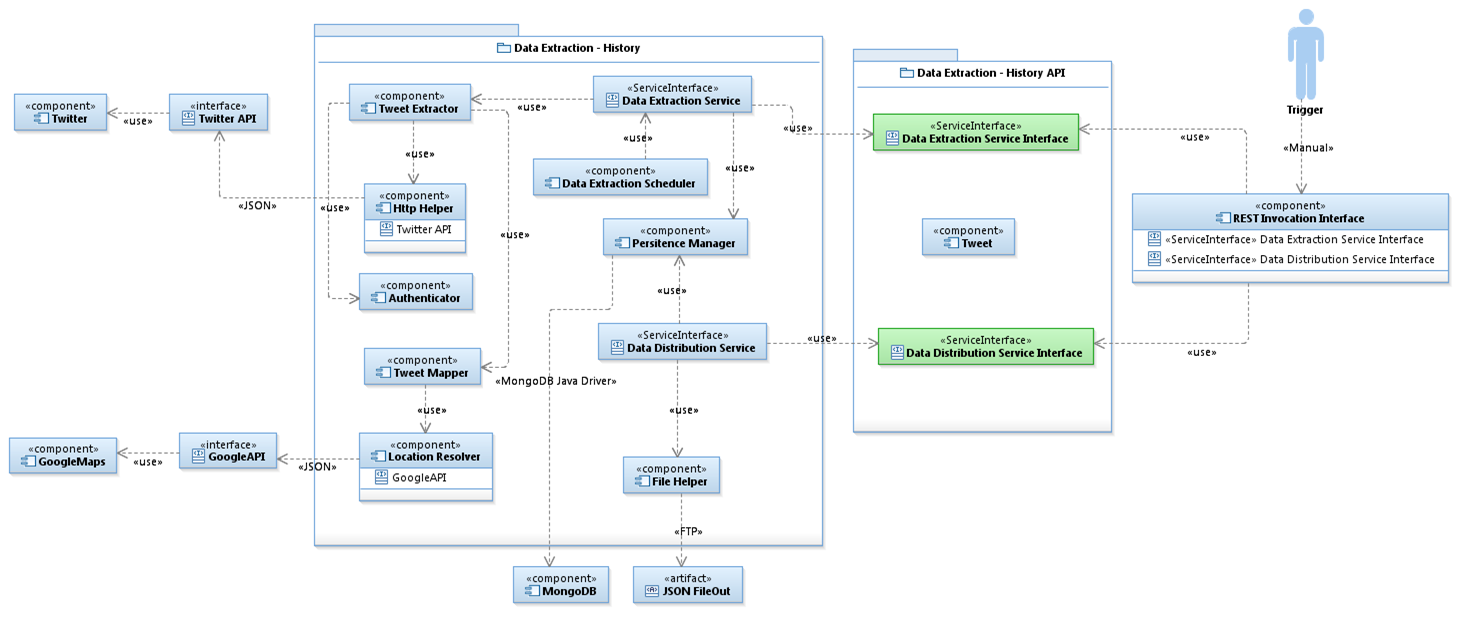
\includegraphics[width=1.2\linewidth]{Batch}}
			\caption{Component Model: History}
			\label{fig:speciation}
		\end{figure}
	
	\subsubsection{Data Acquisition (Streaming)}
	
	Housed in the Application is a Stream Connection Manager, which manages connections to Twitter leveraging off of the 3rd Party Twitter API wrapper called TweetInvi.\\
	\
	\\
	This Connection manager will generate a Twitter Message Handler which will respond to incoming tweets, validate location data with a location verifier component which will consolidate it (if necessary) with the Google Maps API. \\
	\
	\\
	The Twitter Message Handler will then submit a Tweet object to the Database manager to persist it. An Extraction manager can subsequently be used to retrieve the tweets as necessary.
	
		\begin{figure}[H] % Example image
			\center{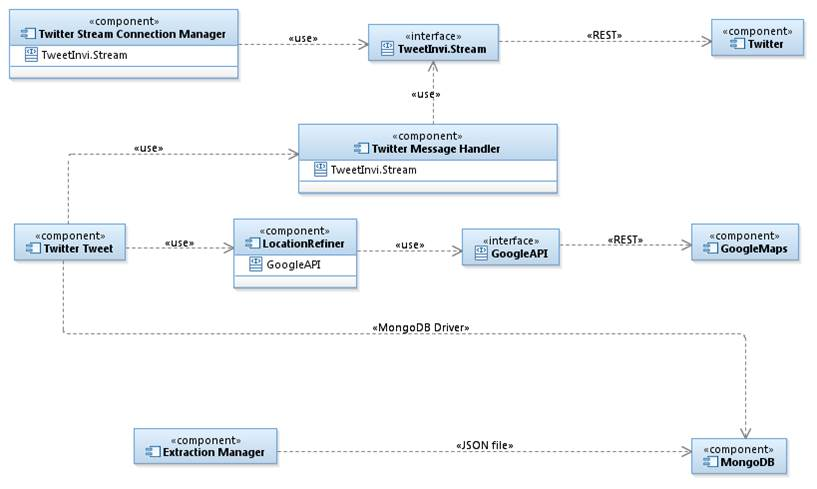
\includegraphics[width=1.15\linewidth]{Streaming}}
			\caption{Component Model: Streaming}
			\label{fig:speciation}
		\end{figure}
	
	\subsubsection{Data Processing}
	
	
	\textbf{Raspberry Pi Cluster - Driver Program:}
	
	\begin{itemize}
		\item The program you write creates an instance of a SparkContext.
		\item  The SparkContext then connects to the Cluster Manager which allocates resources across nodes for the application.
		\item The SparkContext then acquires Executors on Worker Nodes in the cluster, which will run computations and store data for the application hosting the SparkContext.
		\item The application is then sent to the Executors, and then the Tasks that the Executors need to execute are sent through.
		\item 	Executors can communicate with each other using peer-to-peer networking (like bit torrent), in order to transmit shared data (broadcast variables).
		\item Once the Executors have completed their tasks, they communicate back to the Driver Program.
		
	\end{itemize}	
	
	\begin{figure}[H] % Example image
		\center{\includegraphics[width=1.15\linewidth]{MapReduce}}
		\caption{Context Diagram: Data Processing}
		\label{fig:speciation}
	\end{figure}
	

	\textbf{Application Flow (DAG):}
	\\
	\
	\\
	The twitter data is loaded from flat text files, mapped through various functions to strip irrelevant data and transform the text data into Tweet objects. The Tweet objects are then sorted by date. From there, filters are applied to the Tweet objects to only find Tweets for a particular category and hour of day. These results are then summed and reduced to a category count.
	
		\begin{figure}[H] % Example image
			\center{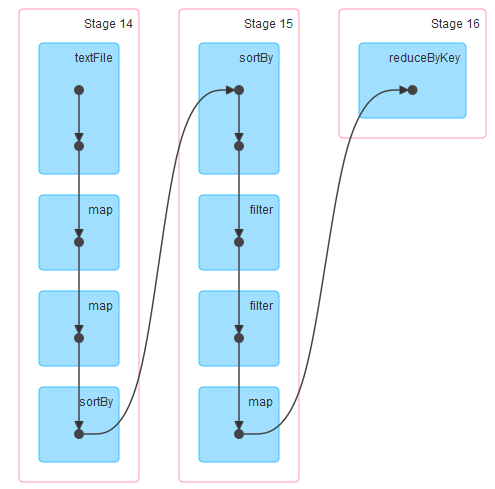
\includegraphics[width=1.0\linewidth]{DAG}}
			\caption{Application Flow}
			\label{fig:speciation}
		\end{figure}
	
	\subsubsection{Data Visualization}
	
	The Visual component implements the MVC pattern to separate the View and controlling logic from the Data. This allows for the data components to be developed separately from the Views. Between the Views and Data Models were Controllers responsible for  loading the views based on the set configuration and provide the views with the required data model.\\
	\\
	The Data Visualisation component was designed to be content agnostic and it allows for the comparison of categories in a topic regardless of the topic or categories.
	All charts were designed to be scalable. All graphs will render as the view point changes allowing for a pleasant user experience.
	
	
		\begin{figure}[H] % Example image
			\center{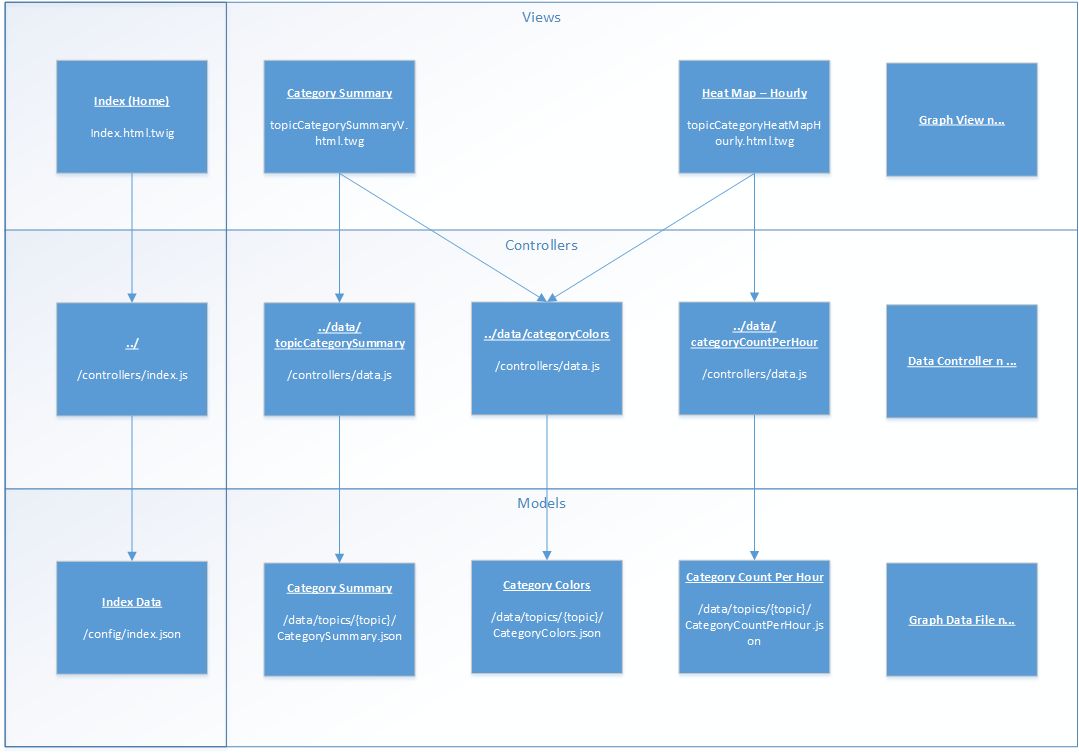
\includegraphics[width=1.15\linewidth]{Visual}}
			\caption{Visualization: MVC Framework}
			\label{fig:speciation}
		\end{figure}
	
	\subsection{Operational Model: Infrastructure Design}
	
	The Raspberry Pi environment is limited in system resources, specifically RAM. It only has 1GB of RAM which is partitioned for use between the system (accessible by the user) and the GPU.\\
	\\
	The Raspberry Pi’s were configured with the least amount of RAM for the GPU (16MB), leaving the remaining space available for user applications. They were not going to run any sort of GUI or windowing system (like the X Window System), so any larger allocation of RAM for GPU use was unnecessary.
	The Raspbian Linux operating system (OS) was installed on the Raspberry Pi’s, as it has been tailored to best utilise the hardware’s resources and features. Further configuration was done on the OS to disable the daemons responsible for controlling the on-board Bluetooth and Wi-Fi modules, thus freeing up even more available RAM.
	Linux’s Network File System (NFS) service was installed and enabled on the Raspberry Pi master node so the slaves in the Spark configuration could operate on a single source of data, with the least amount of memory overhead. When using HDFS, the RAM used by the slave nodes increased from 99MB to 125MB, and from 181MB to 206MB on the master node. In addition to extra RAM use, the time to upload the source data (1GB of plain text files) to HDFS took around 8 minutes, as the data was partitioned across all the data nodes within the cluster.
	
	
	
	
		\begin{figure}[H] % Example image
			\center{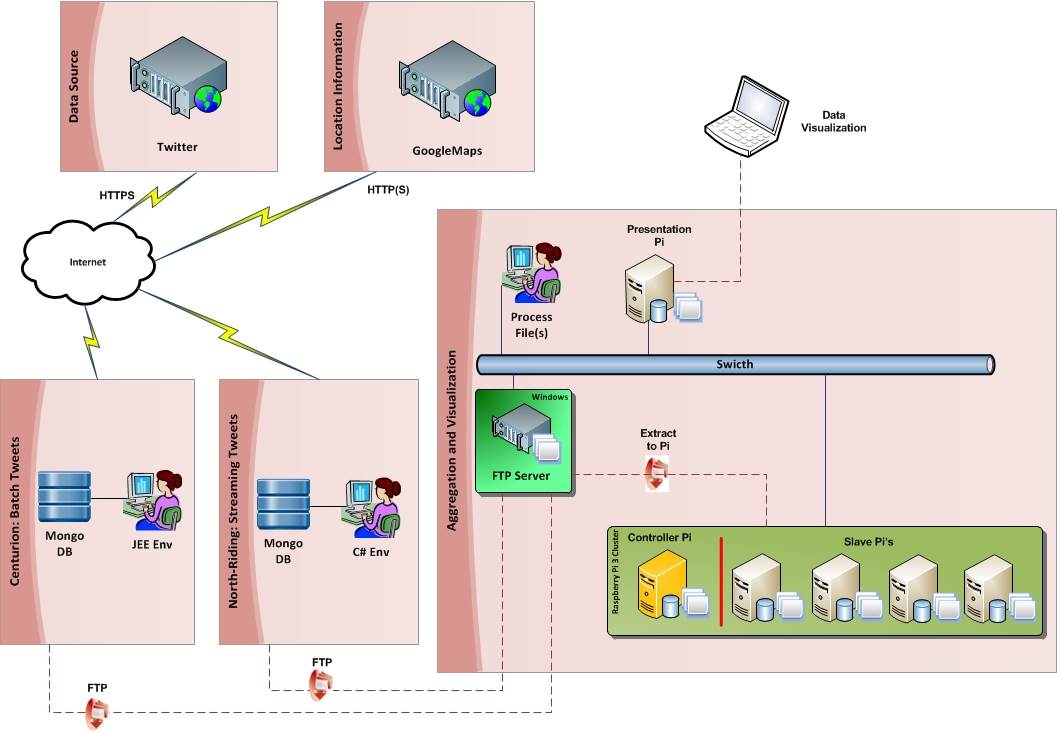
\includegraphics[width=1.15\linewidth]{OM1}}
			\caption{Operational Model: Phyical}
			\label{fig:speciation}
		\end{figure}
		
	
	\subsubsection {Raspberry Pi Configuration Sheet}

	\begin{center}
		\begin{tabular}{ | p{3cm} | p{3cm} | c | c | c |}
			\hline
			\textbf {Node Name} & \textbf {IP Address} & \textbf {Role} & \textbf {OS} & \textbf {Software}  \\
			\hline
			node01 & 192.168.1.200 & Master & Raspbian & Spark\\
			\hline
			node02 & 192.168.1.201 & Slave & Raspbian & Spark\\
			\hline
			node03 & 192.168.1.202 & Slave & Raspbian & Spark\\
			\hline
			node04 & 192.168.1.203 & Slave & Raspbian & Spark\\
			\hline
			node05 & 192.168.1.204 & Slave & Raspbian & Spark\\
			\hline
			dc-pi  & 192.168.1.101 & Web Server & Raspbian & Node.JS\\
			\hline
		\end{tabular}
	\end{center}

	\subsection{Testing Approach}
	
	The major components of the solution were developed independently with very little external real-time integration except for the parts where the solution integrated to external providers - Twitter and GoogleMaps.
	\\
	\\
	The team decided on a testing approach the involved writing software to facilitate a form of automated testing as far as possible. Details of these testing activities can be found in individual reports.
	\\
	\\
	Non-Functional testing was only focused around the Raspberry Pi cluster in order to establish how quickly it can process large sets of twitter data with limited hardware resources for the individual nodes.
	
	\subsection{Possible Extensions}
	
	The project used only Twitter as the Big Data source. According to Statista [7], in April 2016 Facebook ranked number one with 1 590 millions of active users, while Twitter recorded 320 millions of active users. Other social media networking platform ranked included Intagram, WhatsApp, WeChat and LinkedIn among others. Most the social networking service provides an API to retrieve social media messages or posts. The project chose Twitter as the data source because Twitter’s API seemed to be easier to work with. Due to lack of time only one data source was chosen. One of the possible extension in the project lies on the data collection component. The two sub-components can be enhanced to support other social media platforms as the data providers.
	\\
	\\
	Other potential extensions to the solution include developing a smart-phone/ tablet App to make the same sort of analytics reports available to a category of user that is always on the move.
	\\
	\\
	The system itself can in future be hooked into LDAP in order to better control user access and security from a central point as well as ease of provision for new users.
	
	%\subsection{Explanation Summary} %--optional
	
	% Risk - large project given to a small company that is running a core part of the company's systems.
	
	%------------------------------------------------
	
	%\subsubsection{Executive Summary}%--optional
	
	
	%\begin{figure}[H] % Example image
	%	\center{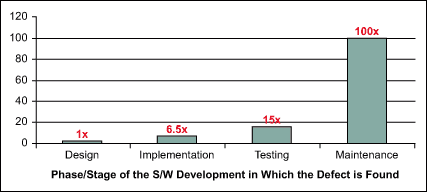
\includegraphics[width=0.55\linewidth]{IBM}}
	%	\caption{Relative Costs to Fix Software Defects (Source: IBM Systems Sciences Institute)}
	%	\label{fig:speciation}
	%\end{figure}
	
	%----------------------------------------------------------------------------------------
	%	CONCLUSION
	%----------------------------------------------------------------------------------------
	
	\section{Conclusion} % Major section
	
	To conclude, Big Data is a resource that no longer needs to be confined to large enterprise processing or expensive computing facilities. There are means by which big data harvesting, transformation and visualisation can be performed using smaller scale endeavours, using open source software and low cost commodity hardware. This conclusion was reached by demonstrating the implementation of low cost hardware and open source software to build a system capable of sourcing tweet data from twitter, transforming the data and providing visualisations that help discern meaningful information about American and South African election trends.
	
	\newpage
	
	%----------------------------------------------------------------------------------------
	%	BIBLIOGRAPHY
	%----------------------------------------------------------------------------------------
	
	\begin{thebibliography}{99} % Bibliography - this is intentionally simple in this template
		
		\bibitem 1 S. Madam. From Databases to Big Data. IEEE Computer Society, 2012.
	
		%\newblock 
		
		\bibitem 2 V. Kumar, R. Yuvaraj, C. Anusha. Effective Distribution of Large Scale Datasets Clustering Based on MapReduce. 2016.
		\bibitem 3 http://www.internetlivestats.com/twitter-statistics/
		
		\bibitem 4 Twitter, "Rate Limits: Chart", https://dev.twitter.com/rest/public/rate-limits, Twitter, San Francisco, Last accessed 29 June 2016.
		
		\bibitem 5 Google, "Google Maps Geocoding API Usage Limits", https://developers.google.com/maps/documentation/geocoding/usage-limits,Googe,San Francisco,Last accessed 29 June 2016.
		
		\bibitem 6 H. Makabee, "Divide-and-Conquer: Coping with Complexity", https://effectivesoftwaredesign.com/2011/06/06/divide-and-conquer-coping-with-complexity/, Last accessed 28 June 2016.
		
		\bibitem 7 Statista, "Leading social networks worldwide as of April 2016, ranked by number of active users (in millions)", 
		http://www.statista.com/statistics/272014/global-social-networks-ranked-by-number-of-users/, Statista Inc, New York, Last accessed 29 June 2016
		
		
		
		%Tweetinvi Twitter Wrapper: https://github.com/linvi/tweetinvi/wiki
		%Google Maps Geocoding API Documentation: https://developers.google.com/maps/documentation/
		%Mongo DB General Tutorials: https://docs.mongodb.com/manual/tutorial/
		%Mongo DB C\# Driver: https://docs.mongodb.com/ecosystem/drivers/csharp/
		%Scala Language Tutorials: http://www.tutorialspoint.com/scala/
		

		
	\end{thebibliography}
	\newpage
	
	\section{Appendices}
	
	\subsection{Appendix A: Time Sheets}
	
	\begin{figure}[H] % Example image
		\center{\includegraphics[width=1.7\linewidth]{Appendix-timesheets}}
		\caption{Group Time Sheet}
		\label{fig:speciation}
	\end{figure}
	
	\newpage
	
	\subsection{Appendix B: Trello Board}
	
	
	\begin{figure}[H] % Example image
		\center{\includegraphics[width=1.15\linewidth]{Appendix-trello}}
		\caption{Trello Board: Project Management}
		\label{fig:speciation}
	\end{figure}
	
	\newpage
	
	\subsection{Appendix C: Slack Dashboard}
	
		
	\begin{figure}[H] % Example image
		\center{\includegraphics[width=1.15\linewidth]{Appendix-slack}}
		\caption{Slack: Team Collaboration}
		\label{fig:speciation}
	\end{figure}
		
		\newpage
	
	\subsection{Appendix D: Git Repository}
	
	A comprehensive list of all the artefacts can be found on GitHub by following the link below:
	\\
	\\
	https://github.com/garethstephenson/ELEN7046\_Group2\_2016\\
	
	
	\newpage
	
	\subsection{Appendix E: List of Technologies and Tools}
	
	 \begin{center}
	 	\begin{tabular}{ | p{3.5cm} | p{12cm} |}
	 		\hline
	 		\textbf{Tool/ Technique} & \textbf{Usage Description} \\
	 		\hline
	 		Trello & Mainly project task allocation to individual team members.\\
	 		\hline
	 		Github & Source control and documentation repository. Also used for online document editing and collaboration.\\
	 		\hline
	 		Slack & Used for online collaboration and communication.\\
	 		\hline
	 		WhatsApp & Used for daily communication with project team members.\\
	 		\hline
	 		Hangouts & Used for online meetings and video conferencing.\\
	 		\hline
	 		Rational Software Architect & Used for architecture deliverables such as Use Cases, Component Models and Sequence Diagrams.\\
	 		\hline
	 		MS Visio & Used for modeling infrastructure deliverables and visualization component model.\\
	 		\hline
	 		MS PowerPoint & Project presentation.\\
	 		\hline
		 	MS Word & Documentation of Individual Reports.\\
		 	\hline
		 	TeXstudio & Group Report construction and online collaboration.\\
		 	\hline
		 	.net C\# Framework version 4.5.2 & Object Oriented Language developed by Microsoft.\\
		 	\hline
		 	Visual Studio Community 2015 & IDE for .net built by Microsoft.\\
		 	\hline
		 	TweetInvi version 0.9.14 & Third Party Wrapper for Twitter.\\
		 	\hline
		 	Mongo DB & Database solution for Persistence.\\
		 	\hline
		 	Mongo DB Driver version 2.2.4 & .net Driver for Mongo DB.\\
		 	\hline
		 	Apache Spark 1.6.1 & Cluster Computing Framework. \\
		 	\hline
		 	Scala 2.10 & Hybrid functional and object oriented programming language.\\
		 	\hline
		 	SBT package manager & Package manager.\\
		 	\hline
		 	JAVA 8 SDK & Java software development kit\\
		 	\hline
		 	IntellijIDE 2016 & Integrated Development Environment.\\
		 	\hline
		 	Raspbian Linux & Raspberry Pi Operating System.\\
		 	\hline
		 
	 	\end{tabular}
	 \end{center}
	 
	 
\begin{center}
	 \begin{tabular}{ | p{3.5cm} | p{12cm} |}
		\hline
	 	\textbf{Tool/ Technique} & \textbf{Usage Description} \\
		\hline
	 	Node.js & Platform that allows for standalone JavaScript application\\
	 	\hline
	 	Node.js Express Framework & Package enabling web features that support MVC implementation.\\
	 	\hline
	 	Node.js - File System & Package enabling File I/O.\\
	 	\hline
	 	Node.js Twig.js & HTML templating engine to allow binding of data to the views.\\
	 	\hline
	 	Bootstrap & UI framework used to aid responsive UI design.\\
	 	\hline
	 	D3 (Data Driven Documents) & A Powerful data visualization component used in the translation of domain data to scalable vector graphics.\\
	 	\hline
	 	Java Enterprise Edition 7 - Jboss Wildfly 10 & Development Framework.\\
	 	\hline
	 	Netbeans 8.1 & Integrated Development Environment.\\
	 	\hline
	 	Apache Maven & Build Tool\\
	 	\hline
	 	Ubuntu Linux 15.10 & Operating System for development and execution of the history component\\
	 	\hline
	 	Test Driven Development & Development technique\\
	 	\hline
	 	\end{tabular}
	\end{center}
		 
	%----------------------------------------------------------------------------------------
	
\end{document}